% =====================================================================
% Clase -- Geometría 7° -- Trimestre I -- Semana 04
% Sesión 004 (mar 22 sep., 6:55, 55 min)
% Tema: Traslaciones
% Subtema: Vector de traslación en la cuadrícula
% Hilo conductor del trimestre I: «Escher: el arte de mover figuras»
% Tema 3 de la guía: Traslaciones (tema:traslaciones)
% Material del docente (no se entrega a los estudiantes).
% =====================================================================
\documentclass[11pt]{article}
\makeatletter\def\input@path{{../../../../../plantillas/estilo/}}\makeatother
\usepackage{mmcantillo}
\guiadelestudiante{../../guia-didactica/guia-periodo-I-transformaciones}

\tipodocumento{Clase}
\asignatura{Geometría}
\titulo{Semana 4: la figura que se desliza}
\grado{7°}
\periodo{I}

% DBA: matematicas grado 7 · DBA 5 — Establece y verifica relaciones de congruencia y
% semejanza entre figuras planas. Evidencia de esta sesión: reconocer que una traslación
% conserva forma, tamaño y orientación, es decir, que la figura trasladada es congruente con
% la original. Se retoma en el tema 6 al componer transformaciones.

\begin{document}

\encabezado*

\begin{center}
{\renewcommand{\arraystretch}{1.3}
\begin{tabularx}{\linewidth}{@{}l l l X l@{}}
  \toprule
  \textbf{Sesión} & \textbf{Fecha} & \textbf{Min} & \textbf{Subtema} & \textbf{Entregables}\\
  \midrule
  004 & mar 22 sep., 6:55 & 55 & Vector de traslación en la cuadrícula & Taller (5 puntos)\\
  \bottomrule
\end{tabularx}}
\end{center}

Tercer paso del hilo. En la sesión anterior el ángulo dejó de ser una abertura quieta y pasó a
medir un giro. Hoy entra el movimiento más sencillo de los tres de Escher: el deslizamiento.
Una baldosa que se repite a lo largo de una pared no gira ni se voltea — solo se corre.
Referencia: \refguia{tema:traslaciones}.

% ---------------------------------------------------------------------
\seccion{Sesión 004 — martes 22 de septiembre · 6:55 · 55 min}

\textbf{Objetivo.} Trasladar figuras en la cuadrícula usando un vector $\langle a, b\rangle$,
deducir el vector a partir de una figura y su imagen, y reconocer que la figura trasladada
conserva forma, tamaño y orientación.

\textbf{Materiales.} Tablero cuadriculado; papel cuadriculado y regla; si se consigue, un
trozo de papel de colgadura o una foto de baldosas repetidas.

\begin{center}
{\renewcommand{\arraystretch}{1.3}
\begin{tabularx}{\linewidth}{@{}l l X@{}}
  \toprule
  \textbf{Momento} & \textbf{Min} & \textbf{Actividad}\\
  \midrule
  Enganche & 0--7 & Mostrar el papel de colgadura (o dibujar tres veces la misma figura
    corrida en el tablero). «¿Qué le hicieron a la figura para que apareciera otra vez?»
    Llegar entre todos a: \emph{la misma distancia, la misma dirección, el mismo sentido}.
    Escher hacía esto a mano, miles de veces.\\
  Definición & 7--18 & El vector $\langle a, b\rangle$: $a$ a la derecha (o a la izquierda si
    es negativo) y $b$ hacia arriba (o abajo). Regla: $(x, y) \mapsto (x+a,\, y+b)$. Hacer
    en el tablero el ejemplo de la guía, triángulo $P(1,1)$, $Q(3,1)$, $R(1,3)$ con
    $\langle 4, 1\rangle$, contando cuadritos y después con la cuenta.\\
  Al revés & 18--28 & La pregunta que cuesta: dada la figura y su imagen, ¿cuál fue el
    vector? Se resta \textbf{imagen menos original}. Hacerlo con un punto y comprobar con
    otro de la misma figura: debe dar el mismo vector. Si no da, alguien se equivocó.\\
  Conservar & 28--35 & Medir con la regla un lado antes y después: mide lo mismo. Las dos
    figuras son \emph{congruentes} y además miran hacia el mismo lado. Contraste rápido:
    si la figura quedara volteada, ya no sería una traslación (eso es la sesión 006).\\
  Taller & 35--52 & Taller individual (5 puntos), en papel cuadriculado.\\
  Cierre & 52--55 & Recoger. Anuncio de la sesión 005: la misma figura, pero girando —
    y por qué la estrella de 16 puntas queda igual cada $22{,}5^\circ$.\\
  \bottomrule
\end{tabularx}}
\end{center}

\textbf{Figura para el tablero: el vector se lee restando.}

\begin{center}
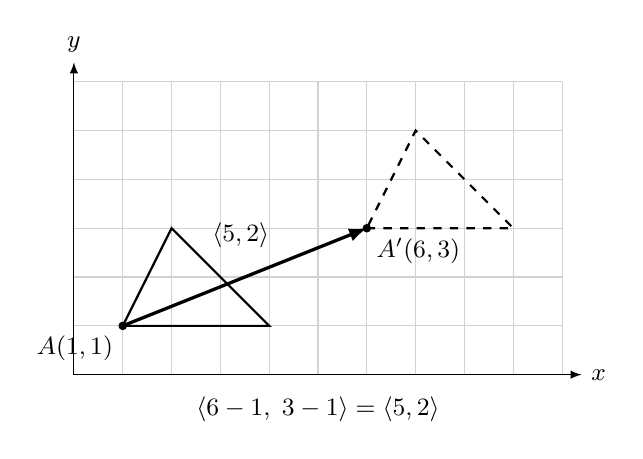
\begin{tikzpicture}[scale=0.62, font=\small, >=latex]
  \draw[gray!35] (0,0) grid (10,6);
  \draw[->] (0,0) -- (10.4,0) node[right] {$x$};
  \draw[->] (0,0) -- (0,6.4) node[above] {$y$};
  \draw[thick] (1,1) -- (4,1) -- (2,3) -- cycle;
  \draw[thick, dashed] (6,3) -- (9,3) -- (7,5) -- cycle;
  \draw[->, very thick] (1,1) -- (6,3);
  \fill (1,1) circle (2.5pt) node[below left] {$A(1,1)$};
  \fill (6,3) circle (2.5pt) node[below right] {$A'(6,3)$};
  \node[above left] at (4.2,2.4) {$\langle 5, 2\rangle$};
  \node at (5,-0.7) {$\langle 6-1,\; 3-1\rangle = \langle 5, 2\rangle$};
\end{tikzpicture}
\end{center}

\begin{nota}
\textbf{Dónde se traban.} En los signos. Trasladar con $\langle 4, -3\rangle$ significa
\emph{bajar} 3, y muchos suben. Ayuda decirlo en voz alta antes de operar: «cuatro a la
derecha, tres para abajo». Y al deducir el vector, el error es restar al revés: conviene fijar
la frase \textbf{«imagen menos original»} y escribirla en el tablero durante toda la sesión.
\end{nota}

\begin{nota}
\textbf{Si el grupo va rápido:} pedir que compongan dos traslaciones seguidas y descubran que
el resultado es una sola traslación (es la pregunta 3 del taller). Si va lento, esa pregunta se
puede terminar en casa.
\end{nota}

\end{document}
